\documentclass[tikz]{standalone}
    \usepackage{tikz}
    \usetikzlibrary{positioning, graphs}
    \usetikzlibrary{graphs.standard}
    \begin{document}
    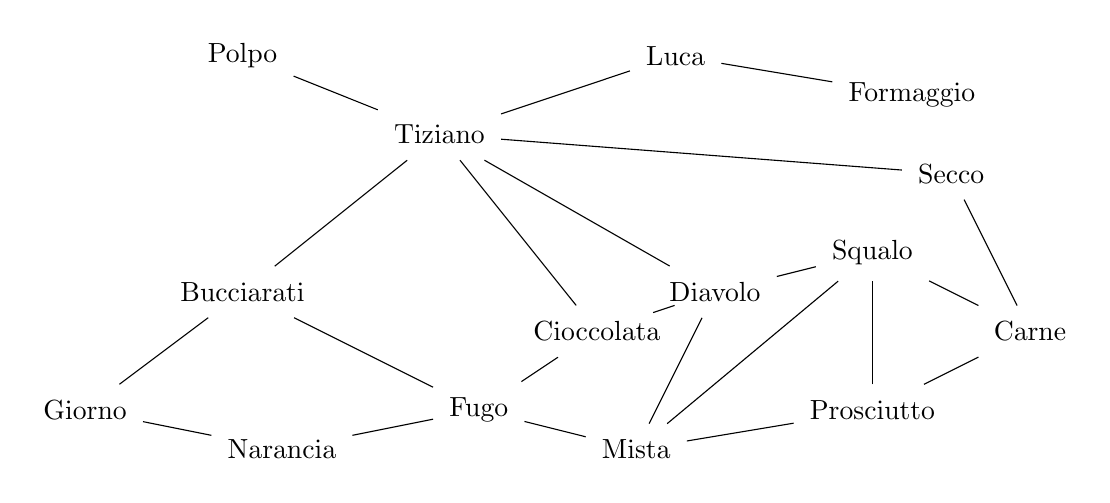
\begin{tikzpicture}
        [vertex/.style={inner sep = 2mm, minimum size = 0.4em},
         edgelabel/.style = {fill = white, inner sep = 0mm, font=\tiny}]
        \node[vertex] (a) at (0,0) {Giorno};
        \node[vertex] (b) at (2.5, -.5) {Narancia};
        \node[vertex] (c) at (5,0) {Fugo};
        \node[vertex] (d) at (7,-.5) {Mista};
        \node[vertex] (e) at (10,0) {Prosciutto};
        \node[vertex] (f) at (2, 1.5) {Bucciarati};
        \node[vertex] (g) at (6.5, 1) {Cioccolata};
        \node[vertex] (h) at (8,1.5) {Diavolo};
        \node[vertex] (i) at (10,2) {Squalo};
        \node[vertex] (j) at (12,1) {Carne};
        \node[vertex] (k) at (4.5,3.5) {Tiziano};
        \node[vertex] (l) at (11,3) {Secco};
        \node[vertex] (m) at (2,4.5) {Polpo};
        \node[vertex] (n) at (7.5,4.5) {Luca};
        \node[vertex] (o) at (10.5,4) {Formaggio};
        
        \draw (a) -- (f);
        \draw (k) -- (f);
        \draw (d) -- (h);
        \draw (c) -- (f);
        \draw (c) -- (b);
        \draw (c) -- (g);
        \draw (h) -- (g);
        \draw (h) -- (k);
        \draw (h) -- (i);
        \draw (e) -- (i);
        \draw (e) -- (j);
        \draw (k) -- (g);
        \draw (k) -- (l);
        \draw (j) -- (l);
        \draw (j) -- (i);
        \draw (k) -- (n);
        \draw (o) -- (n);
        \draw (k) -- (m);
        \draw (c) -- (d);
        \draw (e) -- (d);
        \draw (i) -- (d);
        \draw (a) -- (b);
    \end{tikzpicture}
    \end{document}